\documentclass{article}

\usepackage{graphicx}

\author{Thomas Dizon}
\title{Implementing a Software Rasterizer in C}

\begin{document}

\maketitle

\begin{figure}[h]
	\centering
	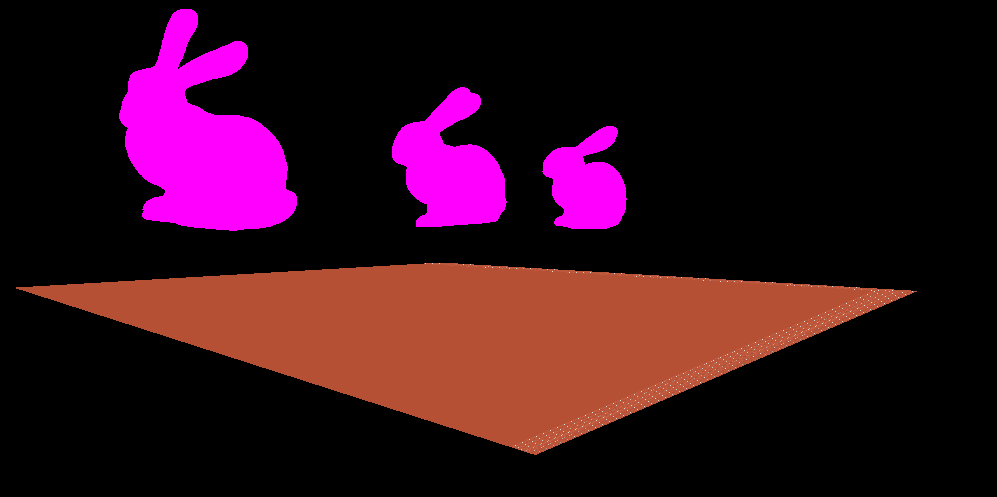
\includegraphics[width=0.6\textwidth]{scene.png}
	\caption{}
\end{figure}

\newpage

\tableofcontents

\newpage

\section{Introduction}

\subsection{Motivation}
* Learn about the Graphics Pipeline
* Help me develop good, optimized, unique graphics in games / game assets
* Learn how the GPU works!

\subsubsection{What is a \textit{Software Rasterizer}?}
* The 'rasterization' step in the graphics render pipline is a specific part which involves converting Primitives into Fragments
* A primitive, in my case, is a Triangle and a Fragment is an (x,y) value on the screen with an additional z value to track its depth
* In the real world, rasterization is done purely through specialized hardware on the GPU (which is why it is so fast)
* To conceptually understand how it works, instead of building a GPU from scratch (hard), I'll use my good old CPU to do the rasterizing (still hard but easier)

\subsubsection{Why \textit{C}?}
* I first touched C during my Systems Programming course at University. It was extrememly difficult for me at the time but very benefiical for my programming skills. I felt that I haven't extracted all that I can from the language yet.
* Also, I wanted to get as low level as possible for this project to ensure I had minimal dependencies. To truly understand the Graphics Pipeline, I wanted to build it truly (well, mostly) from scratch

\subsubsection{What does the project depend on?}
* Right now, it depends on the C standard library, std\_image.h (reference) for dealing with .png files and SDL2 (reference) for handling all the OS level stuff like inputs and writing to the screen. Though you coud easily replace SDL with any other kind of 2D array.

\section{Background}

\subsection{Math Concepts}
\subsubsection{Vectors}
\subsubsection{Matrices}
\subsubsection{Quaternions}
\subsubsection{Transformations}
\subsubsection{Coordinate Systems}

\subsection{Algorithms}
\subsubsection{Rasterization}
* Takes a Primitive (Triangle made of Vertices) after is has been transformed by MVP and VP. It computes Bounding Box and using BaryCentric Coordinates with respect to the Triangle vertex positions decides which pixels to remove based on whether they are inside or outside of the triangle
\subsubsection{Clipping}
\subsubsection{Anti-Aliasing}

\section{System Architecture}

\subsection{Overview}
\subsubsection{System Diagram}
\subsubsection{Project Structure}
\subsubsection{Conventions}

\subsection{Data Design}
\subsubsection{Primitives: Triangles and Vertices}
\subsubsection{Textures and Materials}
\subsubsection{Framebuffer and Zbuffer}
\subsubsection{Scene, GameObject, Camera, LightSource}

\subsection{Software Design}
\subsubsection{Procedural Programming vs. Object Oriented Programming}
* I decided to learn towards a Procedural Programming approach in this project because of the language of choice (C)
* This ended up being a limitation because when I wanted to make the system more complex, it was difficult to refactor and extend

\subsubsection{Graphics Pipeline}

\subsubsection{Scene Management}
\subsubsection{Rendering}
\subsubsection{Shading}

\section{Conclusion \& Future Work}

\subsection{What I learnt}

\subsection{Limitations}

\subsection{A future implementation in C++}


\section{References}

\end{document}

